\documentclass[12pt, a4paper]{article}

% ==================== PACKAGES ====================
\usepackage[utf8]{inputenc}
\usepackage[T1]{fontenc}
\usepackage{times}                    % Times New Roman font (IEEE standard)
\usepackage[margin=1in, headheight=25.2pt]{geometry}   % 1-inch margins
\usepackage{graphicx}                 % For images
\usepackage{booktabs}                 % Professional tables
\usepackage{array}                    % Enhanced table columns
\usepackage{multirow}                 % Multi-row cells in tables
\usepackage{tabularx}                 % Auto-width tables
\usepackage{hyperref}                 % Clickable links
\usepackage{cite}                     % Citation management
\usepackage{amsmath}                  % Math support
\usepackage{amssymb}                  % Math symbols (checkmark)
\usepackage{pifont}                   % Dingbat symbols
\newcommand{\cmark}{\checkmark}       % Checkmark shortcut
\newcommand{\xmark}{\ding{55}}        % Cross mark shortcut
\usepackage{xcolor}                   % Colors
\usepackage{enumitem}                 % Custom lists
\usepackage{caption}                  % Caption formatting
\usepackage{float}                    % Float placement
\usepackage{titlesec}                 % Section title formatting
\usepackage{setspace}                 % Line spacing
\usepackage{fancyhdr}                 % Headers and footers
\usepackage{pdflscape}                % For landscape pages
% ==================== SETTINGS ====================
\hypersetup{
    colorlinks=true,
    linkcolor=black,
    citecolor=black,
    urlcolor=blue
}

% Single spacing (IEEE standard)
\singlespacing

% ---- Page style (IEEE-style header) ----
\pagestyle{fancy}
\fancyhf{}
\fancyhead[L]{\small\textit{ANU --- FACULTY OF COMPUTERS AND DATA SCIENCES, CYBERSECURITY PROGRAM, 2025--2026}}
\fancyfoot[C]{\thepage}
\renewcommand{\headrulewidth}{0.4pt}

% ---- Section formatting (IEEE style - consistent throughout) ----
% Main sections: Roman numeral, centered, uppercase, bold
\titleformat{\section}
  {\normalfont\normalsize\bfseries\centering\MakeUppercase}
  {\Roman{section}.}{0.5em}{}

% Subsections: Letter, bold, left-aligned
\titleformat{\subsection}
  {\normalfont\normalsize\bfseries}
  {\Alph{subsection}.}{0.5em}{}

% Sub-subsections: Numbered, italic, left-aligned
\titleformat{\subsubsection}
  {\normalfont\normalsize\itshape}
  {\arabic{subsubsection})}{0.5em}{}

% Spacing around sections
\titlespacing*{\section}{0pt}{12pt}{6pt}
\titlespacing*{\subsection}{0pt}{10pt}{4pt}
\titlespacing*{\subsubsection}{0pt}{8pt}{4pt}

% Caption formatting (IEEE style)
\captionsetup{
    labelsep=period,
    font=small,
    labelfont=bf,
    textfont=normalfont,
    justification=centering,
    singlelinecheck=false
}

% Rename figure label to "Fig." (IEEE standard)
\renewcommand{\figurename}{Fig.}

% Table caption above, figure caption below (IEEE standard)
\captionsetup[table]{position=above, name=TABLE, labelsep=newline, justification=centering}
\captionsetup[figure]{position=below}

% ==================== TITLE PAGE ====================
\title{\textbf{\Large Threat-Intelligence Based Security Assessment (TIBSA): A Unified Framework for Automated Threat Modeling, Penetration Testing, and Continuous Monitoring}}

% ---- AUTHORS ----
\author{
    Alaa Melook\textsuperscript{1},
    Nadine Rasmy\textsuperscript{2},
    Yumna Medhat\textsuperscript{3},\\
    Rana Ashraf\textsuperscript{4},
    Mahmoud Zaghloula\textsuperscript{5},
    AbdElRahman Hisham\textsuperscript{6}\\[6pt]
    Cybersecurity Program, Faculty of Computers and Data Sciences\\
    Alexandria National University, Alexandria, Egypt\\[4pt]
    {\small\texttt{\textsuperscript{1}2205214@anu.edu.eg,\quad
    \textsuperscript{2}2205203@anu.edu.eg,\quad
    \textsuperscript{3}2205231@anu.edu.eg}}\\
    {\small\texttt{\textsuperscript{4}2205019@anu.edu.eg,\quad
    \textsuperscript{5}2205055@anu.edu.eg,\quad
    \textsuperscript{6}2205032@anu.edu.eg}}\\[10pt]
    \textit{Supervised by:} Dr.~Essam Shaaban
}

\date{}

% ==================== DOCUMENT ====================
\begin{document}

\maketitle
\thispagestyle{fancy}

% ==================== ABSTRACT ====================
\begin{abstract}
Contemporary cybersecurity practices remain largely fragmented, with threat modeling, penetration testing, and threat intelligence typically operating as isolated activities. This fragmentation limits continuous risk visibility and weakens proactive defense capabilities. In this paper, we present the Threat-Intelligence Based Security Assessment (TIBSA) framework, a web-based platform that unifies multi-antivirus scanning, file analysis, STRIDE-based threat modeling, risk-oriented penetration testing, cyber threat intelligence (CTI) enrichment, and continuous monitoring within a scalable, layered cloud-native architecture. TIBSA automates threat-to-test mapping by connecting detected threats to real-world attack techniques through MITRE ATT\&CK integration and external intelligence feeds. The system further incorporates machine learning--assisted detection for phishing and malware classification and dynamic risk scoring based on likelihood and impact. A benchmark evaluation against ten existing security assessment tools demonstrates that TIBSA provides comprehensive coverage across eight key security capabilities---including threat modeling, automation, penetration testing, continuous monitoring, AI/ML integration, SDLC integration, risk prioritization, and threat intelligence---where existing solutions typically address only a subset. The results indicate that TIBSA transforms security assessment from a periodic, reactive exercise into a continuous, adaptive, and data-driven cybersecurity capability.
\end{abstract}

\noindent\textbf{Keywords---}Threat modeling, penetration testing, cyber threat intelligence, multi-antivirus scanning, MITRE ATT\&CK, STRIDE, machine learning, cloud-native security

% ==================== SECTION I: INTRODUCTION ====================
\section{Introduction}

Modern organizations continue to face fragmented cybersecurity practices, where threat modeling, penetration testing, and cyber threat intelligence (CTI) function as isolated activities. The increasing sophistication of adversaries and the rapid expansion of cloud-native infrastructures have amplified the need for continuous, intelligence-driven security validation. Although structured frameworks such as MITRE ATT\&CK~\cite{ref7} and NIST provide systematic guidance for adversary analysis and risk management, operationalizing these standards into a unified, automated security assessment workflow remains a significant challenge. Tools such as OWASP ZAP~\cite{ref5} and MISP address specific stages of the security lifecycle, yet they do not inherently integrate architectural threat analysis, empirical validation, and continuous monitoring within a single adaptive framework. This lack of integration limits continuous risk visibility and weakens proactive defense capabilities.

To address this limitation, this paper introduces the Threat-Intelligence Based Security Assessment (TIBSA) platform, an intelligence-driven framework that unifies automated STRIDE-based threat modeling, risk-oriented penetration testing, CTI enrichment, and continuous monitoring within a scalable, layered cloud-native architecture. By enabling automated threat-to-test mapping, multi-engine analysis, machine learning--assisted detection, and dynamic risk scoring, TIBSA establishes a closed-loop validation mechanism that continuously correlates architectural threats with real-world attack evidence. The proposed approach transforms security assessment from a periodic and reactive exercise into a continuous, adaptive, and data-driven cybersecurity capability.

The remainder of this paper is organized as follows. Section~II defines the research problem. Section~III reviews related work. Section~IV describes the proposed architecture. Section~V presents the validation and benchmark results. Section~VI concludes the paper.

% ==================== SECTION II: RESEARCH PROBLEM ====================
\section{Research Problem}

In recent years, the proliferation of cybersecurity threats has made protecting digital systems and data an increasingly complex challenge. Modern attacks frequently employ advanced malware techniques, including encryption, obfuscation, and polymorphism, which enable malicious software to evade traditional security measures. As a result, many existing protection tools struggle to detect these evolving threats, particularly when they depend on outdated signature databases or a single antivirus engine.

Traditional antivirus solutions that rely on a single scanning engine often fail to accurately detect advanced or zero-day malware. Furthermore, many current malware detection platforms are either proprietary, resource-intensive, or raise privacy concerns when users upload files for scanning. These limitations highlight the need for an integrated approach that combines multiple detection methods within a unified framework.

This paper addresses these challenges by presenting a web-based platform that combines multiple antivirus engines with static file analysis techniques, including hash calculation, entropy measurement, and Portable Executable (PE) header inspection. The system supports secure file uploads, performs hybrid multi-engine scanning, and generates unified reports that include risk assessments. By integrating diverse detection methods, the platform seeks to improve malware identification accuracy while reducing false positives. Additionally, the system preserves user privacy by processing files temporarily and deleting them after analysis. The resulting prototype demonstrates how hybrid malware detection systems can enhance security analysis in academic and small-scale environments.

% ==================== SECTION III: LITERATURE REVIEW ====================
\section{Literature Review}

Recent research in cybersecurity has explored several emerging trends, including automation, artificial intelligence, formal threat modeling, and proactive risk-driven methodologies. These advances aim to address the evolving threat landscape, encompassing insider attacks, information overload in CTI, web application vulnerabilities, critical infrastructure risks, and uncertainty in security decision-making. Key developments include automated correlation of assets to threats, which reduces the workload on analysts; automated generation of executable security tests from threat trees and STRIDE frameworks; machine learning--based behavioral analysis for insider threat identification; risk prioritization through causal graphs; and large language model (LLM)--driven systems for vulnerability coverage and remediation. Collectively, these studies demonstrate the limitations of manual, reactive vulnerability assessment methods and highlight the substantial improvements in efficiency, coverage, and cost-effectiveness achieved through structured automation and intelligent technologies.

\subsection{Automated Cyber Threat Intelligence}

Shin et al.~\cite{ref1} presented the TIME prototype, demonstrating the technical feasibility of automating advanced CTI by linking threats, vulnerabilities, and assets. The system addresses information overload and enables proactive defense through reduced attack surfaces, strengthened defense layers, improved agility, and conformity with NIST standards for critical infrastructure cybersecurity. However, the authors noted that performance optimization is required for large-scale deployment. Overall, the research highlights TIME's potential to support CTI analysts by enabling timely countermeasures and collaborative intelligence sharing against evolving cyber threats.

\subsection{Penetration Testing for Insider Threats}

Through a systematic literature review, Chauhan~\cite{ref2} demonstrated how penetration testing serves as an essential defense against insider threats by enabling comprehensive testing that can be integrated with analytics and training initiatives. The study identified three key findings: the effectiveness of insider behavior simulation, the ongoing challenges associated with resource constraints, and the need for multidisciplinary approaches to address emerging security risks. The author concluded that organizations must conduct regular security assessments using standardized testing techniques and industry-wide collaboration to develop effective security measures.

\subsection{LLM-Based Automated Pentesting}

Huang and Zhu~\cite{ref3} proposed PenHeal, a two-stage LLM framework that autonomously executes penetration tests and generates optimal remediation plans for identified vulnerabilities. Through counterfactual prompting and an Instructor module, PenHeal achieved improvements of 31\% in vulnerability coverage, 32\% in remediation effectiveness, and 46\% in cost reduction compared to baseline methods. This research demonstrates the transformative potential of LLMs for establishing fully automated, end-to-end self-healing cybersecurity systems.

\subsection{Graph-Based Cyber Risk Analysis}

Dekker and Alevizos~\cite{ref4} proposed a methodology for visualizing cyber threats through graph theory to improve decision-making under uncertainty. Their approach involves analyzing adversary behaviors, generating threat scenarios with associated probabilities, and applying established guidelines, including ISO standards, to model uncertainty in risk assessments. Although the methodology requires further validation, it provides guidance for cybersecurity professionals on anticipating and identifying cyber risks while optimizing the use of available intelligence resources in rapidly evolving environments.

\subsection{Web Application Security Testing}

Maniraj et al.~\cite{ref5} evaluated OWASP ZAP as a comprehensive open-source web application vulnerability scanner that automates the identification of vulnerabilities through fuzzing, spidering, and targeted attacks, including SQL injection, cross-site scripting (XSS), and security misconfiguration detection. Their experimental evaluation demonstrated that ZAP improves the identification and remediation of security vulnerabilities, thereby reducing breach risks and delivering actionable insights. The authors concluded that ZAP is an effective solution for proactive web application testing and an essential component of modern DevOps pipelines.

\subsection{Automated Threat Modeling Tools}

Granata and Rak~\cite{ref6} conducted a systematic analysis of automated threat modeling techniques and compared four open-source tools, including PyTM, using a case study based on a WordPress e-commerce website. Their results demonstrate that the demand for automated methods to reduce reliance on domain experts and decrease the time required for threat modeling continues to grow. Although automated tools provide significant improvements over traditional security assessment practices, the authors identified remaining challenges related to scalability, privacy considerations, and integration with hybrid models.

\subsection{Summary of Related Work}

In summary, the reviewed literature demonstrates a clear trend away from manual and static forms of testing toward intelligent, adaptive, and risk-prioritized cybersecurity frameworks through increased automation, predictive intelligence, and AI-assisted decision-making. Although approaches such as PrT-net automated testing, STRIDE-DFD threat modeling, and risk-driven EFSM testing have improved accuracy and efficiency, they frequently require a high degree of modeling expertise and suffer from scalability issues. Similarly, AI-driven frameworks such as TIME and PenHeal achieve automation and predictive intelligence through CTI integration; however, they face challenges related to data quality, computational load, and domain specificity. Additionally, tools such as OWASP ZAP and Next Generation Firewalls demonstrate practical effectiveness but are affected by false positive rates and limited coverage of complex attack vectors. These findings indicate the need for a unified, intelligent framework that connects automated threat modeling to AI-driven prediction and dynamic penetration testing---the objective that TIBSA is designed to address.

% ==================== SECTION IV: PROPOSED ARCHITECTURE ====================
\section{The Proposed Threat-Intelligent Architecture}

This section presents the detailed architecture of the TIBSA platform, organized into eight distinct layers. Each layer represents a logical grouping of components with specific responsibilities, from the user-facing interfaces at the top to the core TIBSA suite at the bottom. The layered design ensures separation of concerns, modularity, and maintainability while enabling seamless data flow and integration between components. Fig.~\ref{fig:architecture} illustrates the overall architecture.

\begin{figure}[H]
\makebox[\linewidth][c]{%
  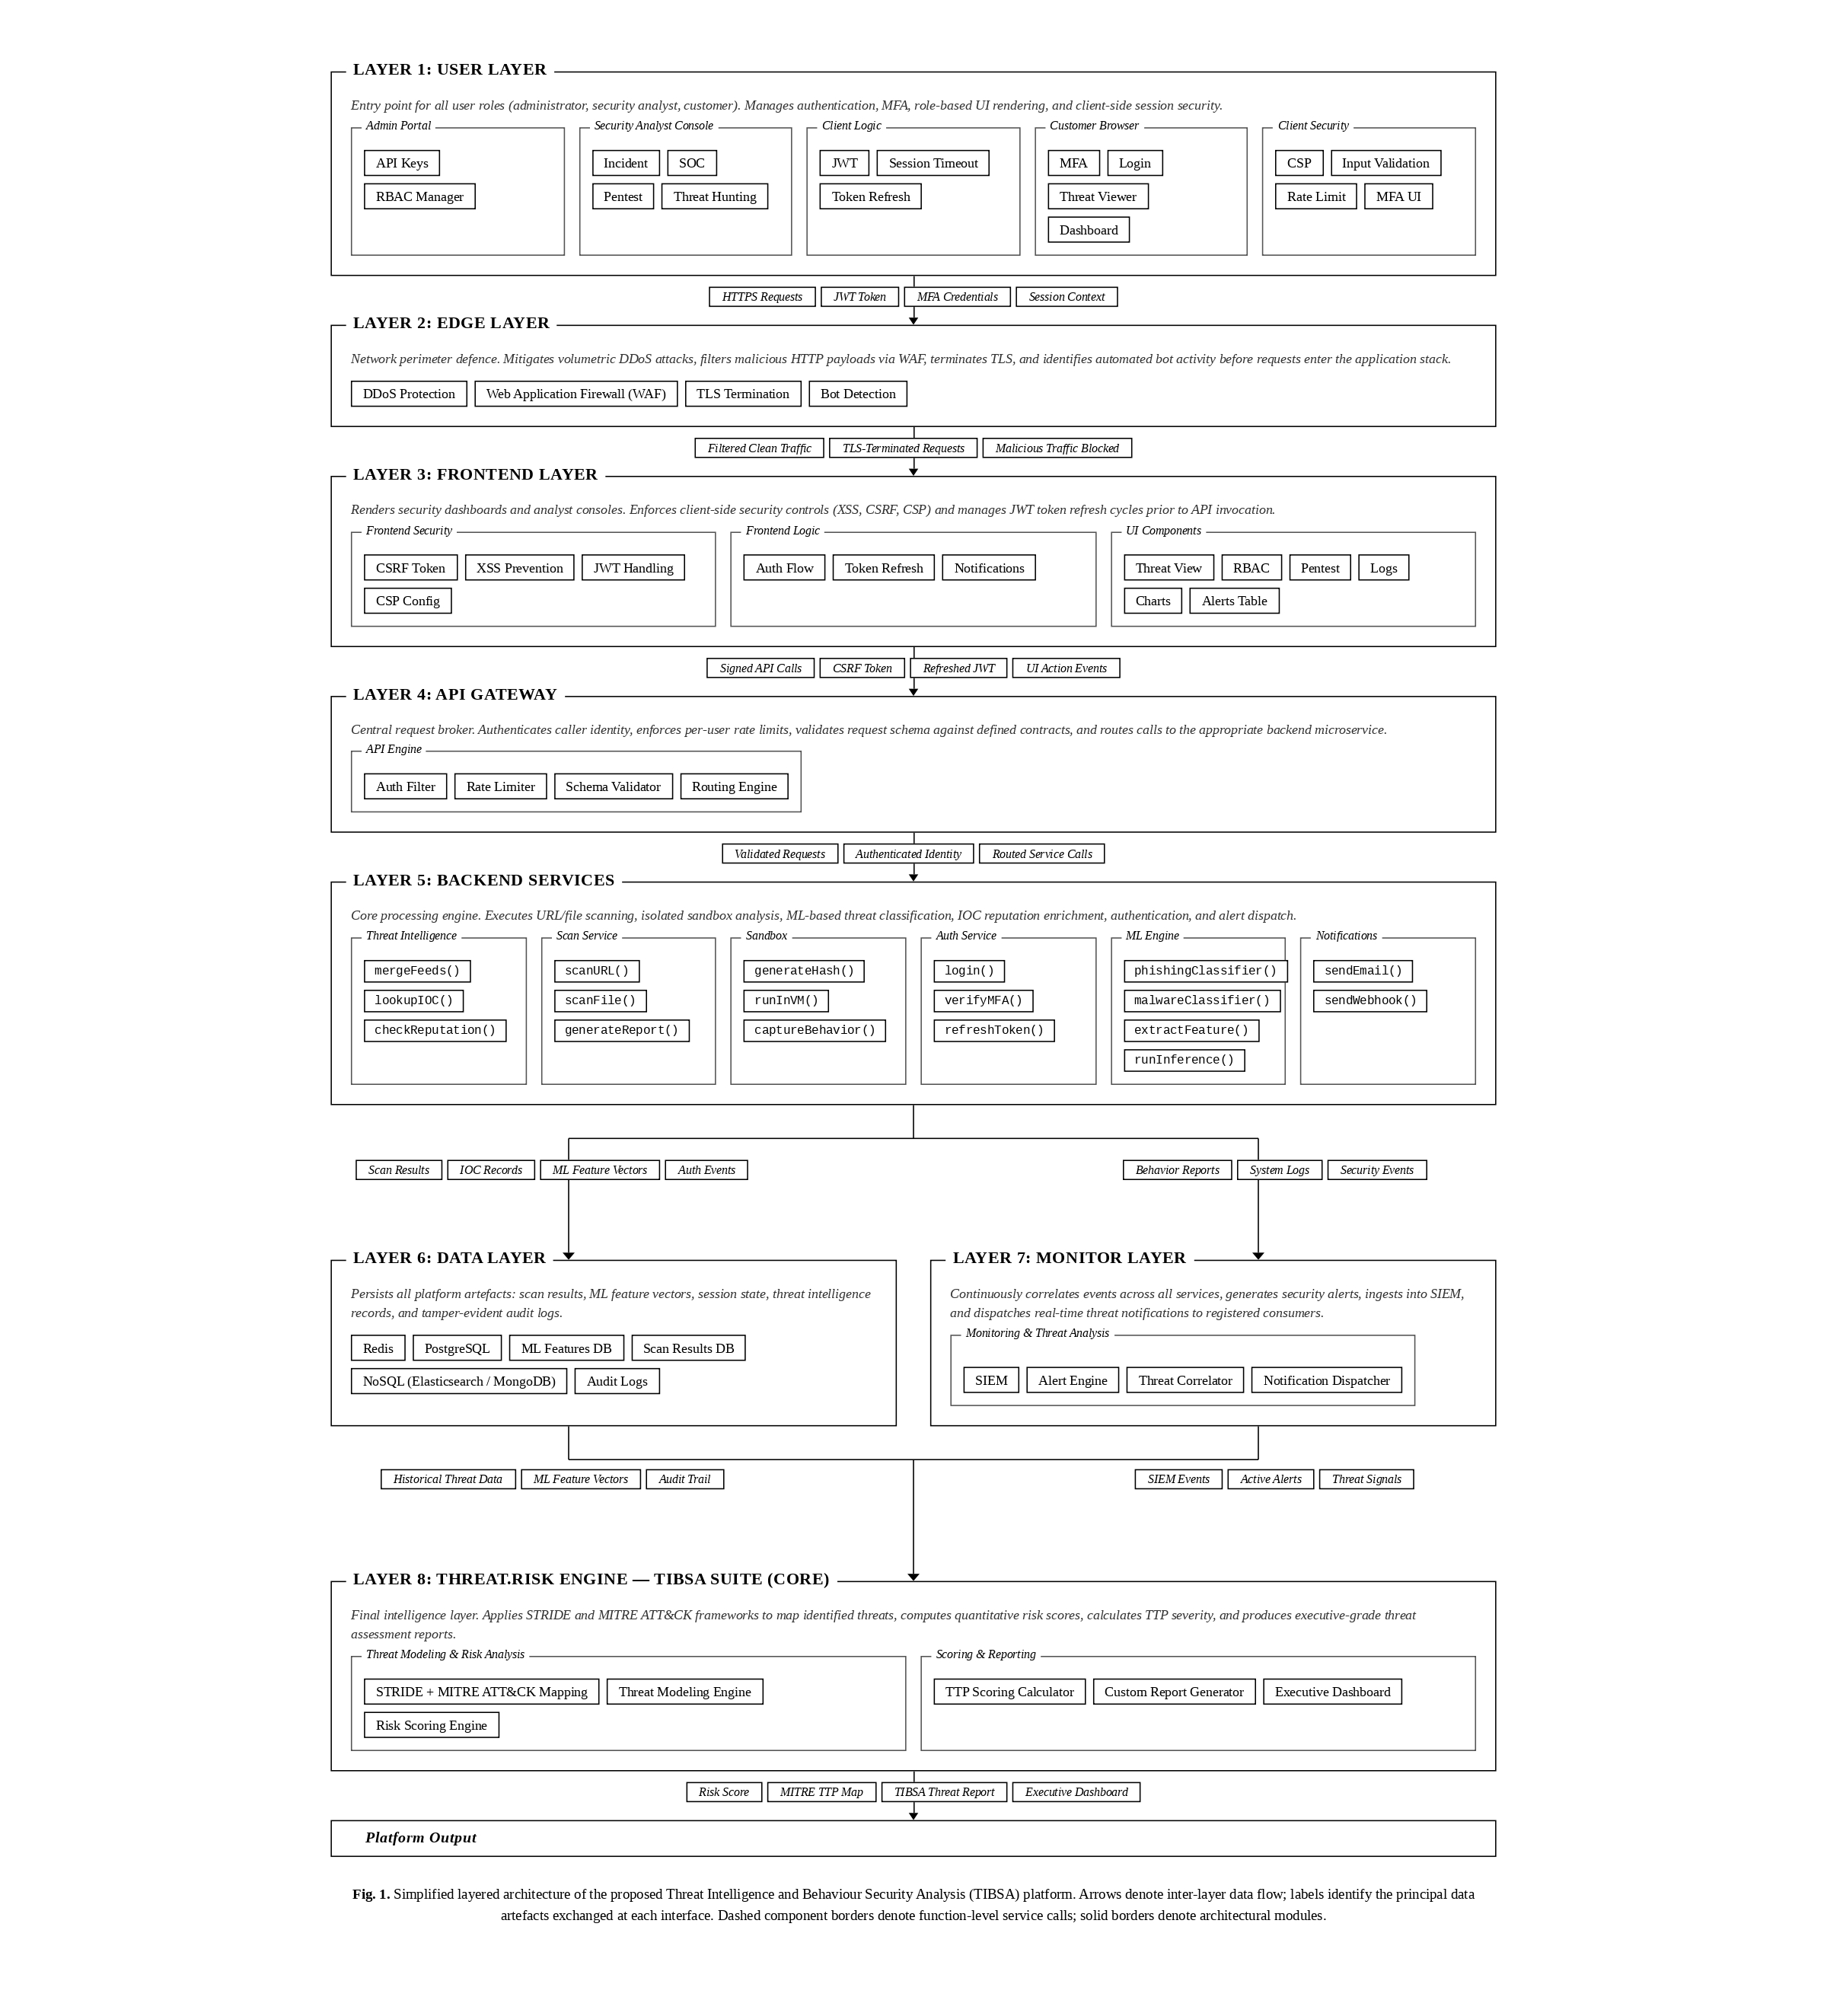
\includegraphics[width=\paperwidth, height=0.92\paperheight, keepaspectratio]{architecture.jpg}%
}
\vspace{1em}
\caption{The proposed TIBSA layered architecture.}
\label{fig:architecture}
\end{figure}

\subsection{User Layer (Layer~1)}

The user layer comprises several sublayers that collectively manage user interaction and client-side security. The Admin Portal provides administrators with API key management and role-based access control (RBAC) configuration capabilities. The Security Analyst Console contains the dashboard for SOC analysts, threat hunters, and penetration testers to access the management interface. The Client Logic Modules sublayer manages user sessions, authentication processes, UI state management based on RBAC, API error handling, and token refresh operations, ensuring the enforcement of client-side security controls. The Customer Browser sublayer hosts the login flow, multi-factor authentication (MFA), threat viewer, and user dashboard. The Client Security sublayer implements multiple layers of protection using browser-native security features and custom validators, including Content Security Policy (CSP), input validation, rate limiting, and MFA UI, serving as the first major security checkpoint in the system.

\subsection{Edge Layer (Layer~2)}

The edge layer performs deep inspection of incoming requests by analyzing patterns associated with common web attacks. The Web Application Firewall (WAF) provides comprehensive protection, including SQL injection detection and blocking, XSS prevention, cross-site request forgery (CSRF) token validation, path traversal detection, and malicious payload filtering. The DDoS Protection component identifies and mitigates abnormal traffic spikes and distributed denial-of-service attacks across OSI Layers~3, 4, and~7. The TLS Termination component serves as the point where encrypted HTTPS traffic is securely decrypted before entering the application stack. The Bot Detection Engine analyzes traffic behavior, device fingerprints, user interaction patterns, request frequency, and known malicious IP ranges to distinguish between human users and automated bots.

\subsection{Frontend Layer (Layer~3)}

The frontend layer encompasses the user-facing interface and the logic that prepares requests before they reach the backend. It handles dashboards, authentication, and penetration testing configuration through three sublayers: Frontend Security, which enforces CSRF token validation, XSS prevention, JSON Web Token (JWT) handling, and CSP configuration; Frontend Logic, which manages authentication flows, token refresh cycles, and notification delivery; and UI Components, which renders the threat view, RBAC controls, penetration testing interface, logs viewer, charts, and alerts table. All requests are secured and properly formatted before transmission to the API Gateway.

\subsection{API Engine (Layer~4)}

The API Gateway serves as the central entry point for all API requests, providing authentication filtering, rate limiting, request schema validation, and intelligent routing to backend microservices. This critical component ensures that only valid, authenticated, and properly formatted requests reach the backend services.

\subsection{Backend Services (Layer~5)}

The backend services layer comprises six sublayers. The Scan Service coordinates security scanning operations for URLs and files, managing the workflow of analyzing potentially malicious content through multiple analysis engines. The Sandbox sublayer isolates and executes potentially malicious content inside a virtual machine, generating hashes, running samples, and capturing behavioral artifacts. The Threat Intelligence Service provides threat enrichment, indicator of compromise (IOC) lookups, and reputation intelligence from multiple sources using MISP and external threat feeds, including VirusTotal, HybridAnalysis, AbuseIPDB, and URLhaus, transforming raw indicators into actionable intelligence. The Auth Service manages user authentication flows, including login, MFA verification, and token refresh operations using Authentik. The ML Engine powers AI-driven threat detection using machine learning models for phishing and malware classification, feature extraction, and model inference. The Notifications sublayer dispatches alerts via email and webhooks to registered consumers.

\subsection{Data Storage Layer (Layer~6)}

The data storage layer manages all persistent data within the platform, including user accounts, scan results, reports, logs, and machine learning data. It employs PostgreSQL for structured relational data, Redis for caching and message queuing, a dedicated ML Features database and Scan Results database, NoSQL storage via Elasticsearch or MongoDB for unstructured and log data, and an Audit Logs store for compliance and forensic trails.

\subsection{Monitoring and Threat Analysis (Layer~7)}

Layer~7 provides continuous security monitoring and threat analysis across the entire platform. It collects logs from all system components---servers, databases, APIs, and edge services---and comprises four components: the Security Information and Event Management (SIEM) module, which ingests and correlates security events; the Alert Engine, which filters and prioritizes generated alerts; the Threat Correlator, which identifies patterns across events; and the Notification Dispatcher, which delivers alerts through dashboards, enabling security and DevOps teams to maintain real-time situational awareness.

\subsection{TIBSA Suite---Core (Layer~8)}

Layer~8 constitutes the core intelligence engine of the platform, automating the entire threat modeling and risk analysis workflow. It is organized into two sublayers: Threat Modeling and Risk Analysis, which encompasses the STRIDE + MITRE ATT\&CK mapping engine, the Threat Modeling Engine, and the Risk Scoring Engine---accepting system architecture details as input, automatically constructing Data Flow Diagrams (DFDs), identifying threats, mapping them to MITRE ATT\&CK techniques, and calculating risk scores based on likelihood and impact; and Scoring and Reporting, which includes the TTP Scoring Calculator, Custom Report Generator, and Executive Dashboard---evaluating existing security controls, prioritizing mitigation actions using cost-benefit analysis, and producing exportable reports with visualizations.

% ==================== SECTION V: VALIDATION ====================
\section{Validation, Discussion, and Benchmark}

To validate the TIBSA framework, a benchmark comparison was conducted against ten existing threat modeling and penetration testing solutions. The evaluation assessed nine security capabilities: Threat Modeling, Automation Level, Penetration Testing, Continuous Monitoring, AI/ML Integration, SDLC Integration, Risk Prioritization, and Threat Intelligence. The results are summarized in Table~\ref{tab:benchmark}.

% ==================== BENCHMARK TABLE ====================
\begin{table}[H]
\centering
\caption{Benchmark Comparison of Security Assessment Solutions}
\label{tab:benchmark}
\small
\renewcommand{\arraystretch}{1.3}
\resizebox{\textwidth}{!}{%
\begin{tabular}{|l|c|c|c|c|c|c|c|c|}
\hline
\textbf{Solution} & \rotatebox{70}{\textbf{Threat Modeling}} & \rotatebox{70}{\textbf{Automation Level}} & \rotatebox{70}{\textbf{Penetration Testing}} & \rotatebox{70}{\textbf{Continuous Monitoring}} & \rotatebox{70}{\textbf{AI/ML Integration}} & \rotatebox{70}{\textbf{SDLC Integration}} & \rotatebox{70}{\textbf{Risk Prioritization}} & \rotatebox{70}{\textbf{Threat Intelligence}} \\
\hline
Microsoft TMT     & \cmark & Medium  & \xmark & \xmark & \xmark & Limited & Basic   & \xmark \\
\hline
Cigent            & \cmark & High    & Limited    & \cmark & Limited    & \cmark & \cmark & \cmark \\
\hline
ThreatModeler     & \cmark & High    & Limited    & \cmark & \xmark & \cmark & \cmark & \cmark \\
\hline
IriusRisk         & \cmark & High    & Via API    & \cmark & Limited    & \cmark & \cmark & \cmark \\
\hline
Threat Dragon     & \cmark & Low     & \xmark & \xmark & \xmark & Limited & Basic   & \xmark \\
\hline
PyTM              & \cmark & High    & \xmark & Limited    & \xmark & \cmark & \cmark & \cmark \\
\hline
Threagile         & \cmark & High    & \xmark & Limited    & \xmark & \cmark & \cmark & Limited \\
\hline
OWASP ZAP         & \xmark & Medium  & \cmark & \cmark & Limited    & \cmark & Basic   & Limited \\
\hline
Metasploit        & \xmark & Medium  & \cmark & \xmark & \xmark & Limited & \xmark & Limited \\
\hline
Nessus            & Limited    & High    & \cmark & \cmark & \xmark & Limited & \cmark & \cmark \\
\hline
\textbf{TIBSA (Proposed)} & \cmark & High & \cmark & \cmark & \cmark & \cmark & \cmark & \cmark \\
\hline
\end{tabular}%
}

\vspace{0.5em}
\noindent\small
\begin{itemize}[nosep, leftmargin=*]
    \item \cmark\ = Fully supported\quad \xmark\ = Not available
    \item Limited = Partial support or requires additional configuration
    \item Basic = Fundamental implementation without advanced capabilities
\end{itemize}
\end{table}

The benchmark results reveal that traditional threat modeling tools such as Microsoft TMT and OWASP Threat Dragon provide STRIDE-based modeling but lack penetration testing capabilities, threat intelligence integration, and continuous monitoring. Similarly, platforms that emphasize automation and SDLC integration offer only limited penetration testing support. In contrast, TIBSA provides a comprehensive solution by unifying threat modeling, penetration testing, threat intelligence, and continuous monitoring within a single framework. TIBSA further enhances threat modeling through STRIDE and MITRE ATT\&CK mapping combined with automated risk scoring, surpassing existing tools that rely on manual effort. The platform achieves a high level of automation, reducing human intervention, and aggregates both internal and external threat intelligence for informed decision-making, complemented by AI and ML models for phishing, malware, and insider threat detection.

These results position TIBSA as an integrative and adaptive cybersecurity framework that not only reduces manual effort but also enables continuous security prioritization and validation across the software development lifecycle.

% ==================== SECTION VI: CONCLUSION ====================
\section{Conclusion}

This paper presented TIBSA, a unified, intelligence-driven cybersecurity framework that integrates automated threat modeling, penetration testing, continuous monitoring, and threat intelligence enrichment within a scalable cloud-native architecture. The benchmark evaluation demonstrated that TIBSA provides comprehensive coverage across key security capabilities where existing tools typically address only a subset. By bridging the gap between fragmented security practices, TIBSA enables organizations to transition from periodic, reactive assessments to continuous, adaptive, and data-driven security validation. Future work will focus on large-scale deployment evaluation, the integration of additional machine learning models for emerging threat categories, and the development of automated compliance mapping to industry standards.

% ==================== REFERENCES ====================
\begin{thebibliography}{9}

\bibitem{ref1}
M.~Alharbi, E.~Al-Shaer, and N.~Almakhdhub, ``Actionable intelligence-oriented cyber threat modeling framework (TIME),'' in \textit{Proc. 55th Hawaii Int. Conf. Syst. Sci. (HICSS)}, Maui, HI, USA, 2022, pp.~1--10.

\bibitem{ref2}
K.~Chauhan, ``Insider threats mitigation: Role of penetration testing,'' Dept. Comput. Sci., Univ. Guelph, Guelph, ON, Canada, Tech. Rep., 2024.

\bibitem{ref3}
J.~Huang and Q.~Zhu, ``PenHeal: A two-stage LLM framework for automated pentesting and optimal remediation,'' \textit{arXiv preprint arXiv:2407.17788}, 2024.

\bibitem{ref4}
M.~Dekker and L.~Alevizos, ``A threat-intelligence driven methodology to incorporate uncertainty in cyber risk analysis and enhance decision making,'' \textit{arXiv preprint}, 2024.

\bibitem{ref5}
S.~P.~Maniraj, C.~S.~Ranganathan, and S.~Sekar, ``Securing web applications with OWASP ZAP for comprehensive security testing,'' \textit{Int. J. Adv. Sig. Img. Sci.}, vol.~10, no.~2, pp.~12--23, 2024.

\bibitem{ref6}
D.~Granata and M.~Rak, ``Systematic analysis of automated threat modelling techniques: Comparison of open-source tools,'' \textit{Softw. Qual. J.}, vol.~32, pp.~125--161, 2024.

\bibitem{ref7}
MITRE Corporation, ``MITRE ATT\&CK,'' 2024. [Online]. Available: \url{https://attack.mitre.org/}

\end{thebibliography}

\end{document}
